\documentclass[11pt]{standalone}
\usepackage{amssymb}
\usepackage{amsmath}
\usepackage[no-math]{fontspec}
\usepackage{unicode-math}
\setmainfont{Libertinus Sans}
\setsansfont{Libertinus Sans}
\setmathfont{Libertinus Math}
\usepackage{pgf,xcolor}
\usepackage{tikz}
\usetikzlibrary{arrows.meta, backgrounds, calc}
\usepackage{pgfplots}
\pgfplotsset{compat=newest}
\usepackage{pifont}

\definecolor{my_darkgray}{HTML}{484949}
\definecolor{my_lightgray}{HTML}{F3F4F4}
\definecolor{my_darkblue}{HTML}{005A94}
\definecolor{my_lightblue}{HTML}{CCDEE9}
\definecolor{my_yellow}{HTML}{FFEC7F}
\definecolor{my_red}{HTML}{E60000}
\definecolor{my_orange}{HTML}{E87846}

\begin{document}
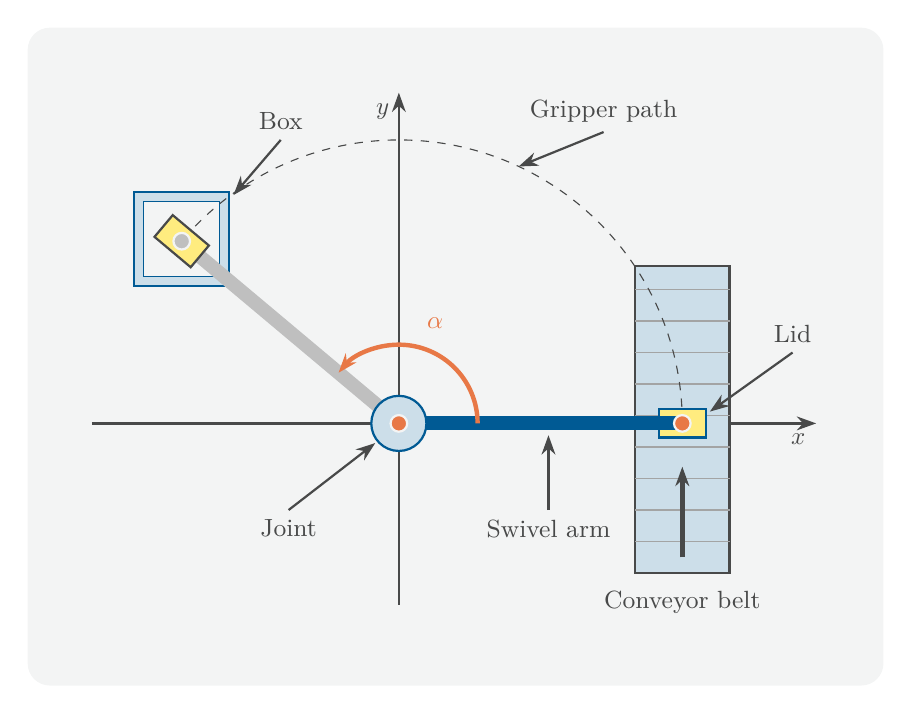
\begin{tikzpicture}[
    show background rectangle,
    background rectangle/.style={fill=my_lightgray, rounded corners=8pt},
    inner frame sep=0.8cm,
    annotation/.style={draw=my_darkgray, thick, -{Stealth[length=7pt, width=5pt]}}
]

    % Draufsicht, Maßstab: 1 m = 6 cm. Gelenk im Ursprung, Armlänge 0.6 m = 3.6 cm,
    % Ablagewinkel 140 Grad, Kistenmitte bei (-0.46 m, 0.39 m)
    \coordinate (G) at (0,0);
    \coordinate (A) at (3.6,0);
    \coordinate (B) at (140:3.6);

    % Koordinatenachsen
    \draw[draw=my_darkgray, thick, -{Stealth[length=7pt, width=5pt]}] (-3.9,0) -- (5.3,0)
        node[anchor=north east, font=\small, text=my_darkgray] {$x$};
    \draw[draw=my_darkgray, thick, -{Stealth[length=7pt, width=5pt]}] (0,-2.3) -- (0,4.2)
        node[anchor=north east, font=\small, text=my_darkgray] {$y$};

    % Förderband mit Rollen und Transportrichtung
    \draw[fill=my_lightblue, draw=my_darkgray, thick] (3.0,-1.9) rectangle (4.2,2.0);
    \foreach \y in {-1.5,-1.1,...,1.8} {
        \draw[draw=my_darkgray!50, thin] (3.0,\y) -- (4.2,\y);
    }
    \draw[draw=my_darkgray, ultra thick, -{Stealth[length=7pt, width=5pt]}] (3.6,-1.7) -- (3.6,-0.55);
    \node[font=\small, text=my_darkgray, anchor=north] at (3.6,-2.0) {Conveyor belt};

    % Kiste mit Wand
    \draw[fill=my_lightblue, draw=my_darkblue, thick] (-3.36,1.74) rectangle (-2.16,2.94);
    \draw[fill=my_lightgray, draw=my_darkblue, thin] (-3.24,1.86) rectangle (-2.28,2.82);

    % Greiferbahn
    \draw[draw=my_darkgray, thin, dashed] (3.6,0) arc[start angle=0, end angle=140, radius=3.6];

    % Schwenkarm in Ablagestellung (blass) mit abgelegtem Deckel
    \draw[draw=my_darkgray!35, line width=5pt, line cap=round] (G) -- (B);
    \draw[fill=my_yellow, draw=my_darkgray, thick, rotate around={140:(B)}]
        ($(B)+(-0.3,-0.18)$) rectangle ($(B)+(0.3,0.18)$);
    \draw[fill=my_darkgray!35, draw=my_lightgray, thick] (B) circle (3pt);

    % Schwenkarm in Grundstellung über dem Deckel auf dem Band
    \draw[fill=my_yellow, draw=my_darkblue, thick] (3.3,-0.18) rectangle (3.9,0.18);
    \draw[draw=my_darkblue, line width=5pt, line cap=round] (G) -- (A);
    \draw[fill=my_orange, draw=my_lightgray, thick] (A) circle (3pt);

    % Sockel mit Gelenk
    \draw[fill=my_lightblue, draw=my_darkblue, thick] (G) circle (0.35);
    \draw[fill=my_orange, draw=my_lightgray, thick] (G) circle (3pt);

    % Schwenkwinkel alpha
    \draw[draw=my_orange, ultra thick, -{Stealth[length=7pt, width=5pt]}]
        (1.0,0) arc[start angle=0, end angle=140, radius=1.0];
    \node[font=\small, text=my_orange] at (70:1.35) {$\alpha$};

    % Beschriftungen
    \draw[annotation] (-1.4,-1.1) -- (-0.3,-0.25);
    \node[font=\small, text=my_darkgray, anchor=north] at (-1.4,-1.1) {Joint};
    \draw[annotation] (1.9,-1.1) -- (1.9,-0.15);
    \node[font=\small, text=my_darkgray, anchor=north] at (1.9,-1.1) {Swivel arm};
    \draw[annotation] (5.0,0.9) -- (3.95,0.15);
    \node[font=\small, text=my_darkgray, anchor=south] at (5.0,0.9) {Lid};
    \draw[annotation] (-1.5,3.6) -- (-2.1,2.9);
    \node[font=\small, text=my_darkgray, anchor=south] at (-1.5,3.6) {Box};
    \draw[annotation] (2.6,3.7) -- (65:3.6);
    \node[font=\small, text=my_darkgray, anchor=south] at (2.6,3.7) {Gripper path};

\end{tikzpicture}
\end{document}
